\documentclass{article}

\usepackage{fancyhdr}
\usepackage{extramarks}
\usepackage{amsmath}
\usepackage{amsthm}
\usepackage{amsfonts}
\usepackage{tikz}
\usepackage[plain]{algorithm}
\usepackage{algpseudocode}
\usepackage{graphicx}
\usepackage{gensymb}
\usepackage{calc}
\usepackage[framed,numbered,autolinebreaks,useliterate]{mcode}
\usepackage{listings}
\usepackage{empheq}
\usepackage{enumitem}
\usepackage[font=footnotesize]{caption}

\graphicspath{{./images/}}

\usetikzlibrary{automata,positioning}

%
% Basic Document Settings
%

\topmargin=-0.45in
\evensidemargin=0in
\oddsidemargin=0in
\textwidth=6.5in
\textheight=9.0in
\headsep=0.25in

\linespread{1.1}

\pagestyle{fancy}
\lhead{\hmwkAuthorName}
\chead{\hmwkClass\ \hmwkTitle}
\rhead{\firstxmark}
\lfoot{\lastxmark}
\cfoot{\thepage}

\renewcommand\headrulewidth{0.4pt}
\renewcommand\footrulewidth{0.4pt}

\setlength\parindent{0pt}

%
% Create Problem Sections
%

\newcommand{\enterProblemHeader}[1]{
    \nobreak\extramarks{}{Problem {#1} continued on next page\ldots}\nobreak{}
    \nobreak\extramarks{{#1} (continued)}{{#1} continued on next page\ldots}\nobreak{}
}

\newcommand{\exitProblemHeader}[1]{
    \nobreak\extramarks{{#1} (continued)}{{#1} continued on next page\ldots}\nobreak{}
    % \stepcounter{#1}
    \nobreak\extramarks{{#1}}{}\nobreak{}
}

\setcounter{secnumdepth}{0}
\newcounter{partCounter}

\newcommand{\problemNumber}{0.0}

\newenvironment{homeworkProblem}[1][-1]{
    \renewcommand{\problemNumber}{{#1}}
    \section{\problemNumber}
    \setcounter{partCounter}{1}
    \enterProblemHeader{\problemNumber}
}{
    \exitProblemHeader{\problemNumber}
}

%
% Homework Details
%   - Title
%   - Class
%   - Author
%

\newcommand{\hmwkTitle}{Homework\ \#6}
\newcommand{\hmwkClass}{RBE 500}
\newcommand{\hmwkAuthorName}{\textbf{Arjan Gupta}}

%
% Title Page
%

\title{
    \vspace{2in}
    \textmd{\textbf{\hmwkClass\ \hmwkTitle}}\\
    \vspace{3in}
}

\author{\hmwkAuthorName}
\date{}

\renewcommand{\part}[1]{\textbf{\large Part \Alph{partCounter}}\stepcounter{partCounter}\\}

%
% Various Helper Commands
%

% Useful for algorithms
\newcommand{\alg}[1]{\textsc{\bfseries \footnotesize #1}}

% For derivatives
\newcommand{\deriv}[2]{\frac{\mathrm{d}}{\mathrm{d}#2} \left(#1\right)}

% For compact derivatives
\newcommand{\derivcomp}[2]{\frac{\mathrm{d}#1}{\mathrm{d}#2}}

% For partial derivatives
\newcommand{\pderiv}[2]{\frac{\partial}{\partial #2} \left(#1\right)}

% For compact partial derivatives
\newcommand{\pderivcomp}[2]{\frac{\partial #1}{\partial #2}}

% Integral dx
\newcommand{\dx}{\mathrm{d}x}

% Alias for the Solution section header
\newcommand{\solution}{\textbf{\large Solution}}

% Probability commands: Expectation, Variance, Covariance, Bias
\newcommand{\E}{\mathrm{E}}
\newcommand{\Var}{\mathrm{Var}}
\newcommand{\Cov}{\mathrm{Cov}}
\newcommand{\Bias}{\mathrm{Bias}}

\newlength\dlf% Define a new measure, dlf
\newcommand\alignedbox[2]{
% Argument #1 = before & if there were no box (lhs)
% Argument #2 = after & if there were no box (rhs)
&  % Alignment sign of the line
{
\settowidth\dlf{$\displaystyle #1$}  
    % The width of \dlf is the width of the lhs, with a displaystyle font
\addtolength\dlf{\fboxsep+\fboxrule}  
    % Add to it the distance to the box, and the width of the line of the box
\hspace{-\dlf}  
    % Move everything dlf units to the left, so that & #1 #2 is aligned under #1 & #2
\boxed{#1 #2}
    % Put a box around lhs and rhs
}
}

\begin{document}

\maketitle

\nobreak\extramarks{Question 1}{}\nobreak{}

\pagebreak

\begin{homeworkProblem}[Question 1]
    Consider the following robot joint model
    \[J\ddot{\theta}(t) + B\dot{\theta}(t) = u(t) + d(t)\]
    where $J$ is the inertia of the link, $B$ is the effective damping on the link, $\theta$ is the joint angle, $u$ is 
    the actuator torque (input), and $d$ is the disturbance acting on the system.
    \vspace{0.15in}\\
    First, assume that disturbance is zero and take \(J = 2\), \(B = 0.5\). Design a PD 
    controller such that the closed loop system is critically damped, and settling time is 2 second. Do 
    not do this by tuning the gains;  calculate  the  $K_p$  and  $K_d$  gains  using  natural  frequency  and 
    damping ratio.

    \subsection{Solution}
    Since $d(t) = 0$, \(J = 2\), \(B = 0.5\), we have

    \[2 \ddot{\theta}(t) + 0.5 \dot{\theta}(t) = u(t)\]

    Transform to Laplace domain,

    \begin{align*}
        2 \Theta(s) s^2 + 0.5 \Theta(s) s &= U(s)
    \end{align*}
    \begin{equation}
        \Theta(s) [2s^2 + 0.5s] = U(s)
    \end{equation}
    \begin{align*}
        \frac{\Theta(s)}{U(s)} = \frac{1}{2s^2 + 0.5s}
    \end{align*}

    Let our PD controller model be
    \[K_p e + K_d \dot{e} = u\]
    Transform to Laplace domain,
    \begin{align*}
        K_p E(s) + K_d E(s) s &= U(s)\\
        E(s) [K_p + K_d s] &= U(s)
    \end{align*}
    Therefore, the transfer function for the PD controller is
    \begin{equation}
        \frac{U(s)}{E(s)}=K_p + K_d s
    \end{equation}

    Now we can draw the block diagram, as shown below.

    \begin{figure}[h]
        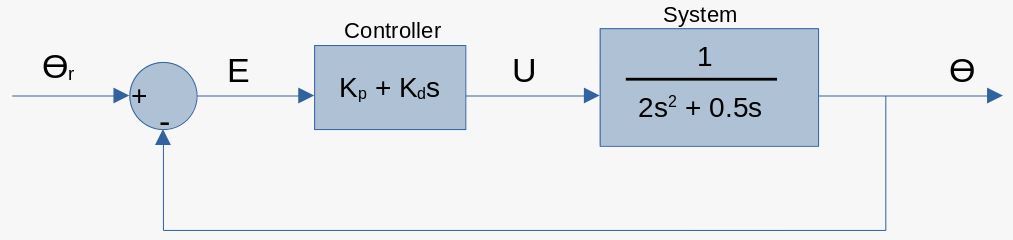
\includegraphics[scale=0.4]{q1-closed-loop-sys.png}
        \centering
    \end{figure}

    From the block diagram, we can see that
    \[E = \Theta_r - \Theta\]

    Using equation 2,

    \[\frac{U(s)}{K_p + K_d s} = \Theta_r - \Theta\]

    Furthermore, using equation 1,

    \begin{align*}
        \frac{\Theta(s) [2s^2 + 0.5s]}{K_p + K_d s} &= \Theta_r - \Theta\\
        \frac{\Theta[2s^2 + 0.5s]}{K_p + K_d s} + \Theta &= \Theta_r\\
        \Theta \left(\frac{2 s^2 + 0.5 s}{K_p + K_d s} + 1\right) &= \Theta\\
        \Theta\left(\frac{2 s^2 + 0.5 s + K_p + K_d s}{K_p + K_d s}\right) &= \Theta_r\\
    \end{align*}
    Therefore,
    \[
        \frac{\Theta}{\Theta_r}=\frac{K_p + K_d s}{2 s^2 + s(0.5 + K_d) + K_p}
    \]

    So our charateristic equation is,
    \begin{align*}
        2 s^2 + s(0.5 + K_d) + K_p = 0\\
        s^2 + s\frac{(0.5 + K_d)}{2} + \frac{K_p}{2} = 0
    \end{align*}

    The general form of the charateristic equation is
    \[s^2 + (2\xi\omega_n)s + {\omega_n}^2 = 0\]
    Where $\xi$ is the damping ratio and $\omega_n$ is the natural frequency.
    \vspace*{0.3in}\\
    Hence, we have,
    \begin{equation}
        {\omega_n}^2 = \frac{K_p}{2}
    \end{equation}
    and
    \begin{equation}
        2\xi\omega_n = \frac{(0.5 + K_d)}{2}
    \end{equation}

    Also, we know that the natural frequency and settling time $T_s$ are related by

    \[\xi\omega_n T_s = 4\]

    Since we are solving for a critically damped system, we set \(\xi = 1\). We also want settling time $T_s$ = 2 seconds.\\

    So, \begin{align*}
        \xi\omega_n T_s &= 4\\
        1 \cdot \omega_n \cdot 2 &= 4\\
        \omega_n &= 2
    \end{align*}

    Plugging this into equation 3, we have

    \begin{align*}
        {(2)}^2 &= \frac{K_p}{2}\\
        4 &= \frac{K_p}{2}\\
        \alignedbox{K_p}{=8}
    \end{align*}

    Also, plugging in values into equation 4, we have

    \begin{align*}
        2(1)(2) &= \frac{0.5 + K_d}{2}\\
        8 &= 0.5 + K_d\\
        \alignedbox{K_d}{=7.5}
    \end{align*}
\end{homeworkProblem}

\nobreak\extramarks{Question 2}{}\nobreak{}

\pagebreak

\begin{homeworkProblem}[Question 2]
    Follow steps in the assignment PDF file. Explain the process and be sure to include the plot to your report.
    \vspace{0.2in}

    \subsection{Solution}

    First we write the following MATLAB script that contains the system and controller values of the closed loop system. 
    Here, $J$ is the intertia of the link in the system model, $B$ is the effective damping on the link in the system model,
    $K_p$ is the proportional gain for the controller, and $K_d$ is the derivative gain for the controller.

    \lstinputlisting{hw6_q2.m}

    \vspace{0.15in}

    Next, we run our script so that the variables are loaded into our base workspace in MATLAB.\@ We then type \lstinline{simulink}
    into the MATLAB command window to launch Simulink. Now we use the Library Browser to begin to construct our closed-loop block diagram.
    Our process is as follows:
    \vspace{0.15mm}
    \begin{itemize}
        \item First, we choose the step function as the input block. We double-click on this block and set the step time as 0 instead of 1, because we want to provide an instantaneous signal.
        \item Then we choose gain blocks to construct our PD controller. By double-clicking on the gain blocks, we are able to indicate 
        the variables \lstinline{K_p} and \lstinline{K_d} from our base worksapce. In the case of \lstinline{K_d}, we also add a derivative
        block before the gain block.
        \item Now we add a summation block to add these gains.
        \item Next, we add a transfer function block and write $[J \hspace{1mm} B \hspace{1mm} 0]$ in the denominator to accurately represent our transfer function.
        \item Now we connect the output of the controller summation into our system model.
        \item We can now add a scope to monitor the output of our controlled system. We connect the transfer function output to the scope.
        \item Now we add a summation after the input, and edit 22it by double-clicking the summation and making sure it says $| \hspace{1mm} + \hspace{1mm} -$.
        \item We can now represent our feedback error. For this, we right-click the connector leading to the scope, and draw a line into the minus part of the summation after the input.
        \item The input is fed into the plus part of the summation right after the input, so we draw that connector.
        \item The output of the summation right after the input feeds into our controller, so we draw that connector as well.
        \item We are almost ready to run our simulation. However as explained in the lectures, in order to be more accurate, we want to edit the solver 
        in our model settings such that the solver-selection is fixed-step, and ode3 (Bogacki-Shampine).
        \item Now our closed loop system is ready to run. We click the play button to run the simulation.
        \item Our plot is now ready, which can be viewed by double-clicking the scope block.
    \end{itemize}

    \vspace{0.15in}

    Figure 1 below shows the end-result of the closed loop system we constructed in Simulink.

    \begin{figure}[h!]
        \centering
        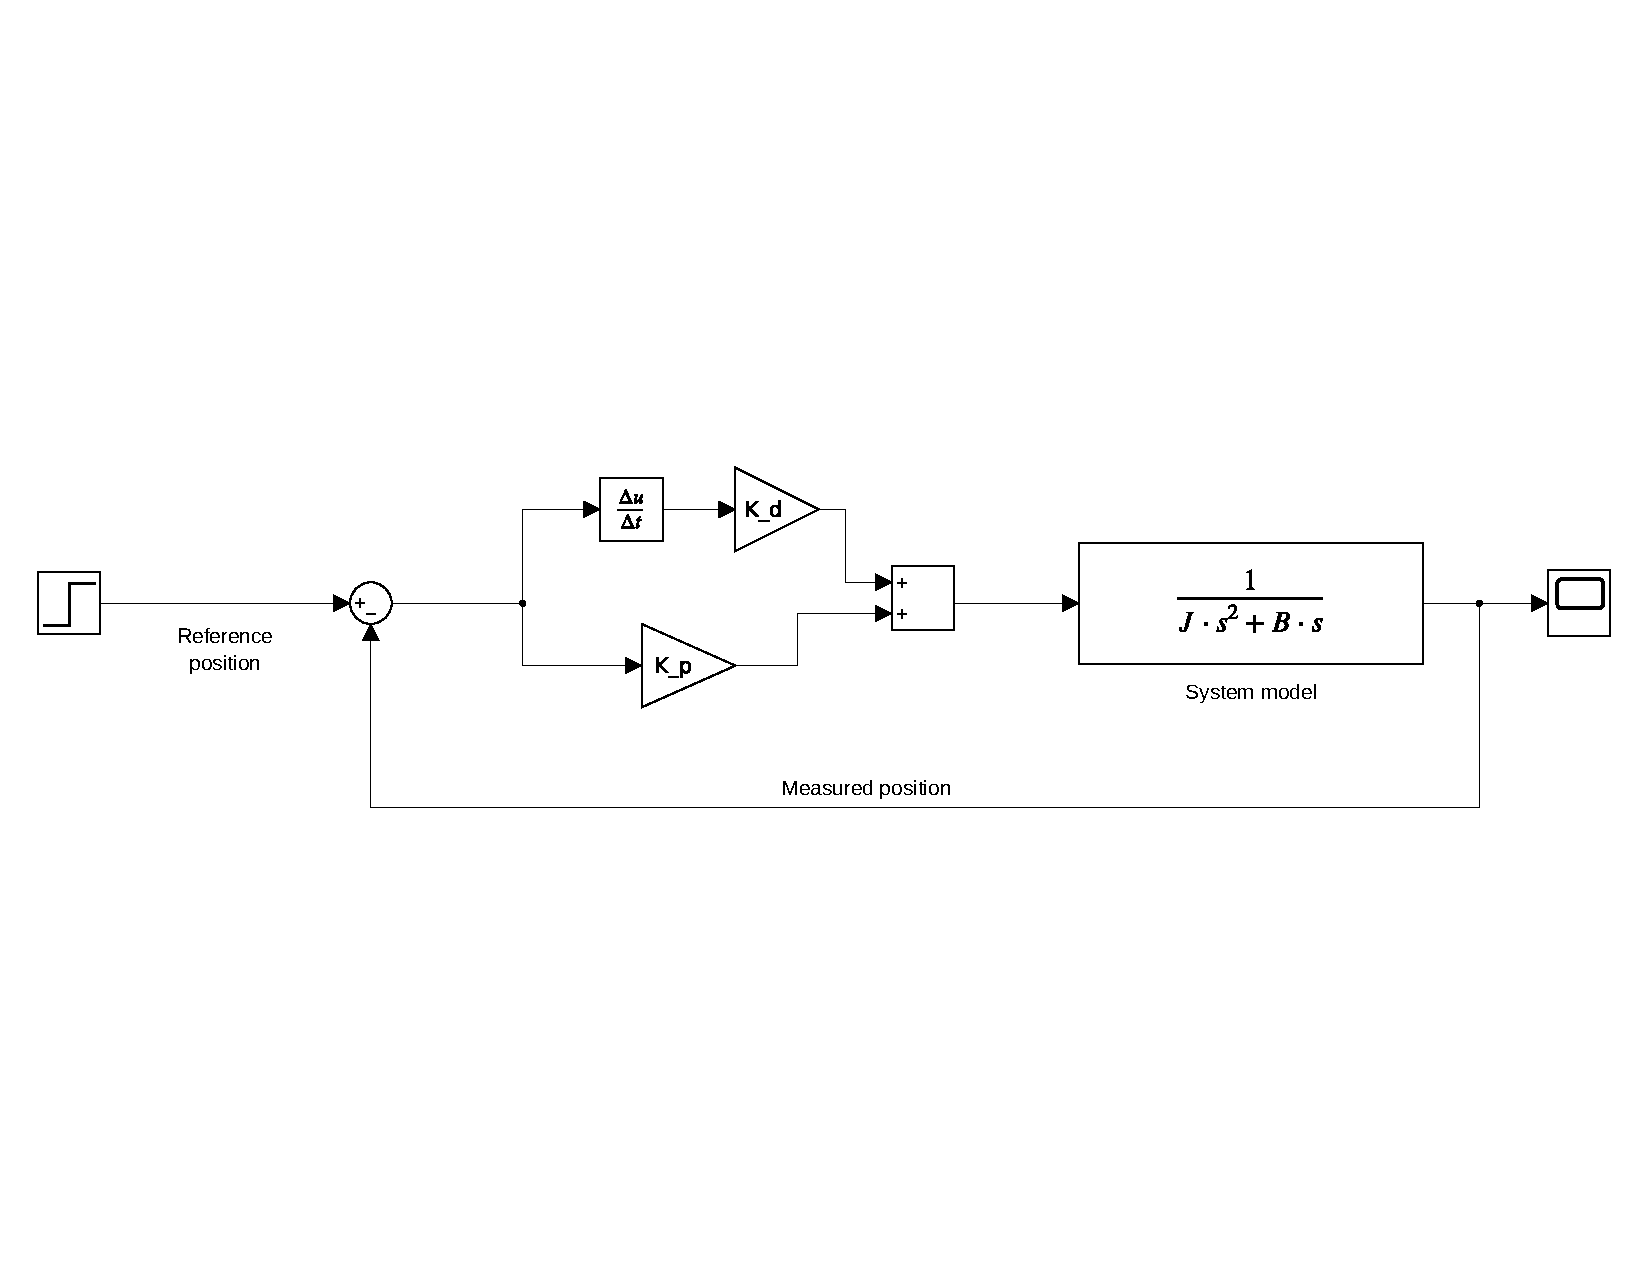
\includegraphics[scale=0.59]{hw6-q2-block-diagram.pdf}
        \vspace*{-7mm}
        \caption{Block diagram for Question 2}
    \end{figure}

    \vspace{0.15mm}
    After constructing the block diagram, we obtained the following plot (Figure 2).

    \begin{figure}[h]
        \centering
        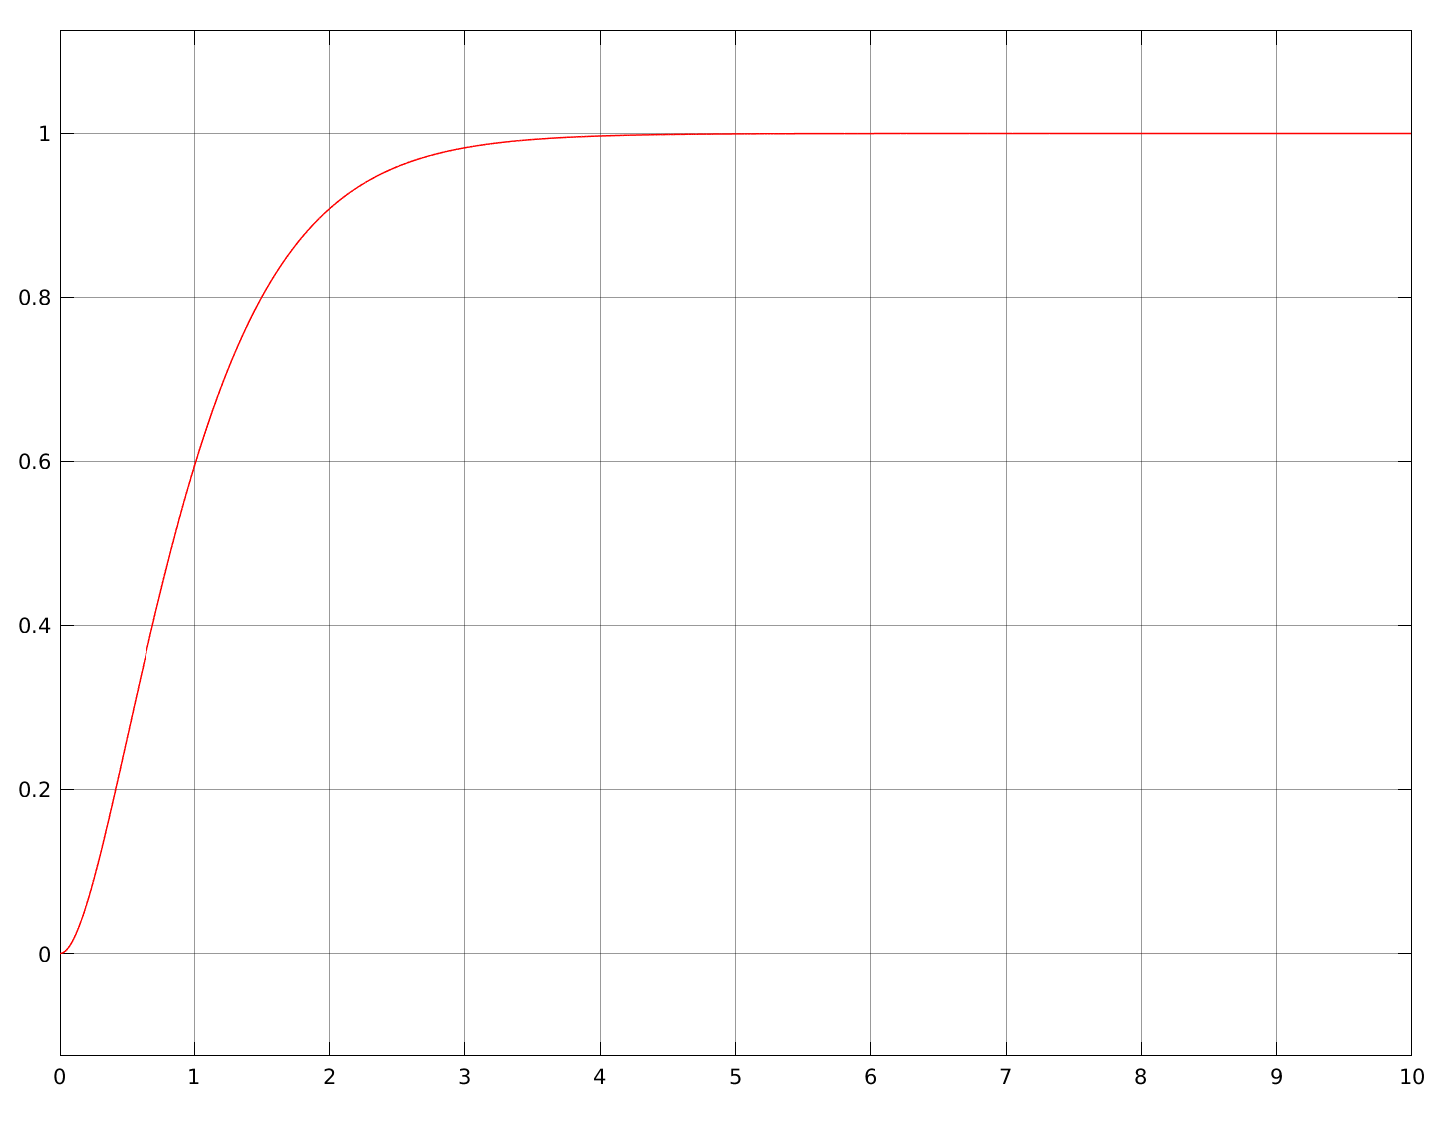
\includegraphics[scale=0.5]{hw6_q2_figure}
        \vspace*{-2mm}
        \caption{Generated plot for Question 2}
    \end{figure}
\end{homeworkProblem}

\nobreak\extramarks{Question 3}{}\nobreak{}

\pagebreak

\begin{homeworkProblem}[Question 3]

    You may have noticed that the system performance (overshoot and 
    settling  time)  is  quite  close  to  your  goal,  but  it  might  not  be  exactly  there.  Report  the  current 
    settling time in your report (you may need to zoom in to the plot to see the exact settling time). 
    This  is  because  the  equations  defining  the  relations  between  the  damping  ratio,  natural 
    frequency, settling time and overshoot, are approximations, not exact relations. Specifically, the 
    settling time equation is only accurate when damping ratio is $\ll 1$. Now, tune the values of $K_p$ 
    and $K_d$ so that you get closer to your goal performance. Please remember the $K_p$ and $K_d$ to the 
    system  performance  from  our  slides  and  discussions.  Explain  your  process  and  include  a  plot 
    showing the results after tuning. If your values have already been good and do not require tuning, 
    report that as well.

    \subsection{Solution}

    When we zoom into the plot we obtained in Question 2, we get the following plot (Figure 3).

    \begin{figure}[h]
        \centering
        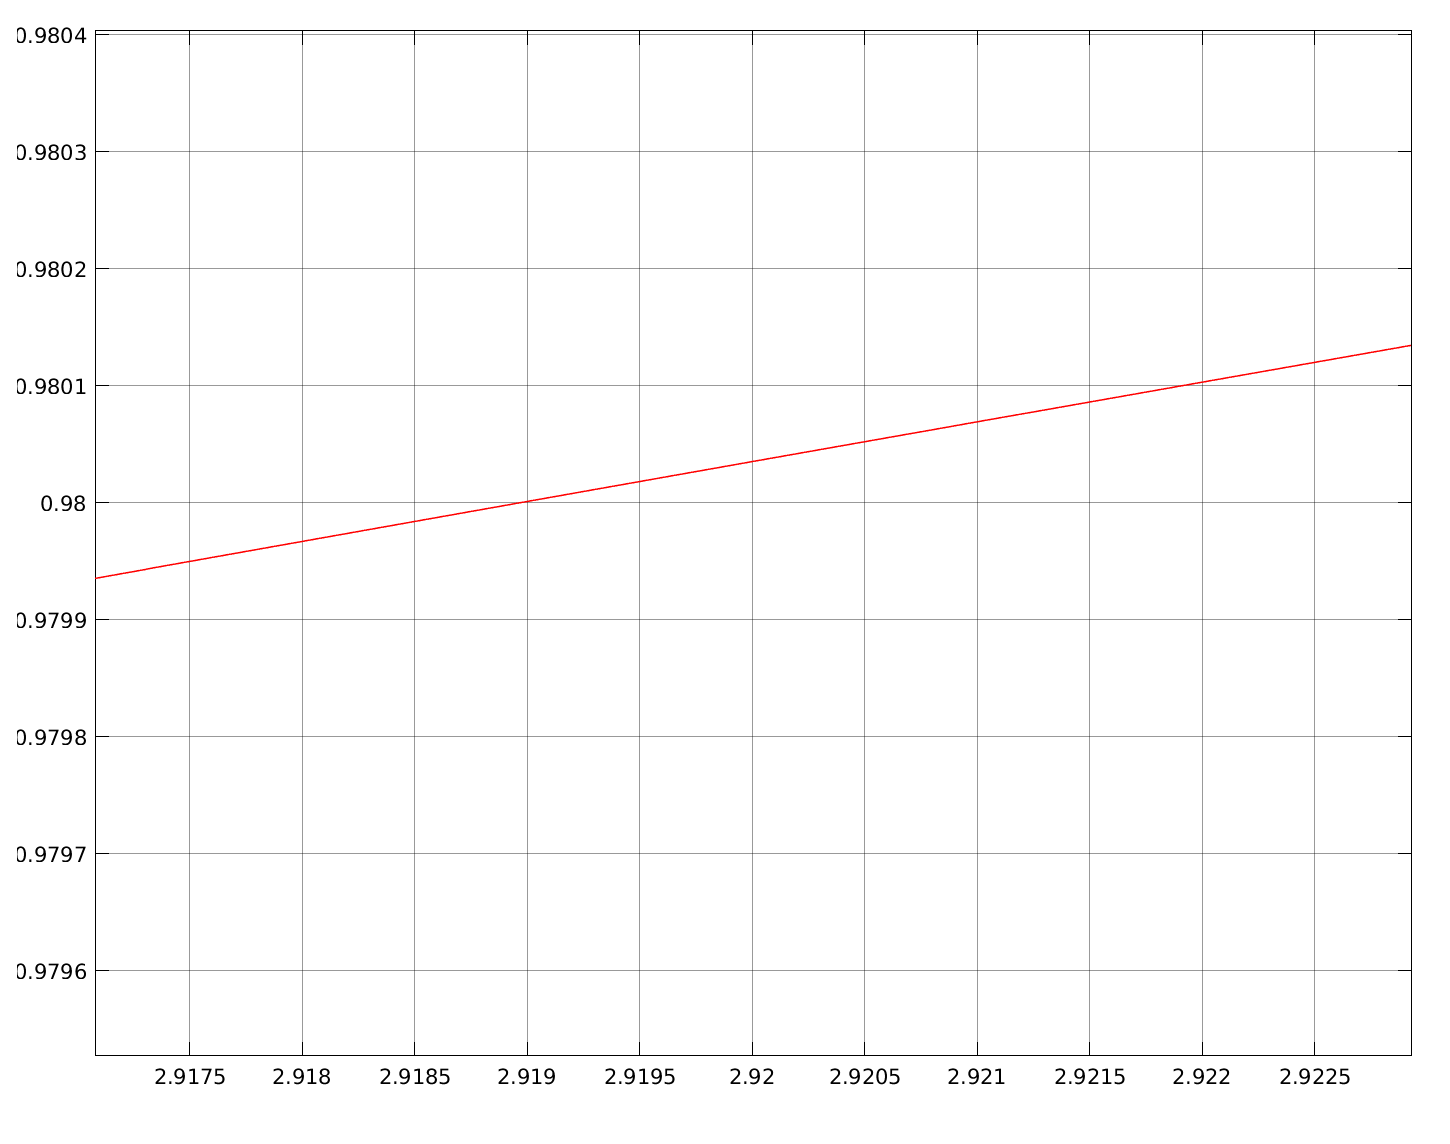
\includegraphics[scale=0.5]{hw6_q3_graph}
        \vspace*{-2mm}
        \caption{Zoomed-in plot for Question 3}
    \end{figure}

    It is clear from this plot that the system's response enters the 2\% tolerance zone (i.e., above 0.98 and below 1.02) at 4.2 seconds.
    Therefore, the settling time $T_s$ is 2.919 seconds.\\
    \vspace{0.05in}\\
    Now we take the following steps to manually tune our $K_p$ and $K_d$ values to achieve our goal settling time of 2 seconds.

    \begin{itemize}
        \item First $K_p$ was increased to 10. This decreased the settling time to about 2.2 seconds with no overshoot.
        \item Then $K_p$ was incrased to 12. This decreased the settling time to about 1.6 seconds but introduced an overshoot of about 1\%.
        \item $K_p$ was reduced to 11. This decreased the settling time to 1.8, and reduced overshoot to 0.5\%.
        \item Next, we increased $K_d$ to 15. This drastically worsened our settling time (around 4 sec) while removing the overshoot.
        \item $K_d$ was then decreased to 6. This decreased our settling time to 1.3, and caused an overshoot of 5\%.
        \item We then set $K_d$ to 8. This decreased our overshoot to about 0.1\%, and decreased our settling time to 2.034 seconds.
    \end{itemize}

    Therefore, by tuning our controller gains to \(\boxed{K_p = 11}\) and \(\boxed{K_d = 8}\), we have achieved an improved controller.\\
    \vspace{0.1in}\\
    The following plots show the improved system response and settling-time of the system.

    \begin{figure}[h]
        \centering
        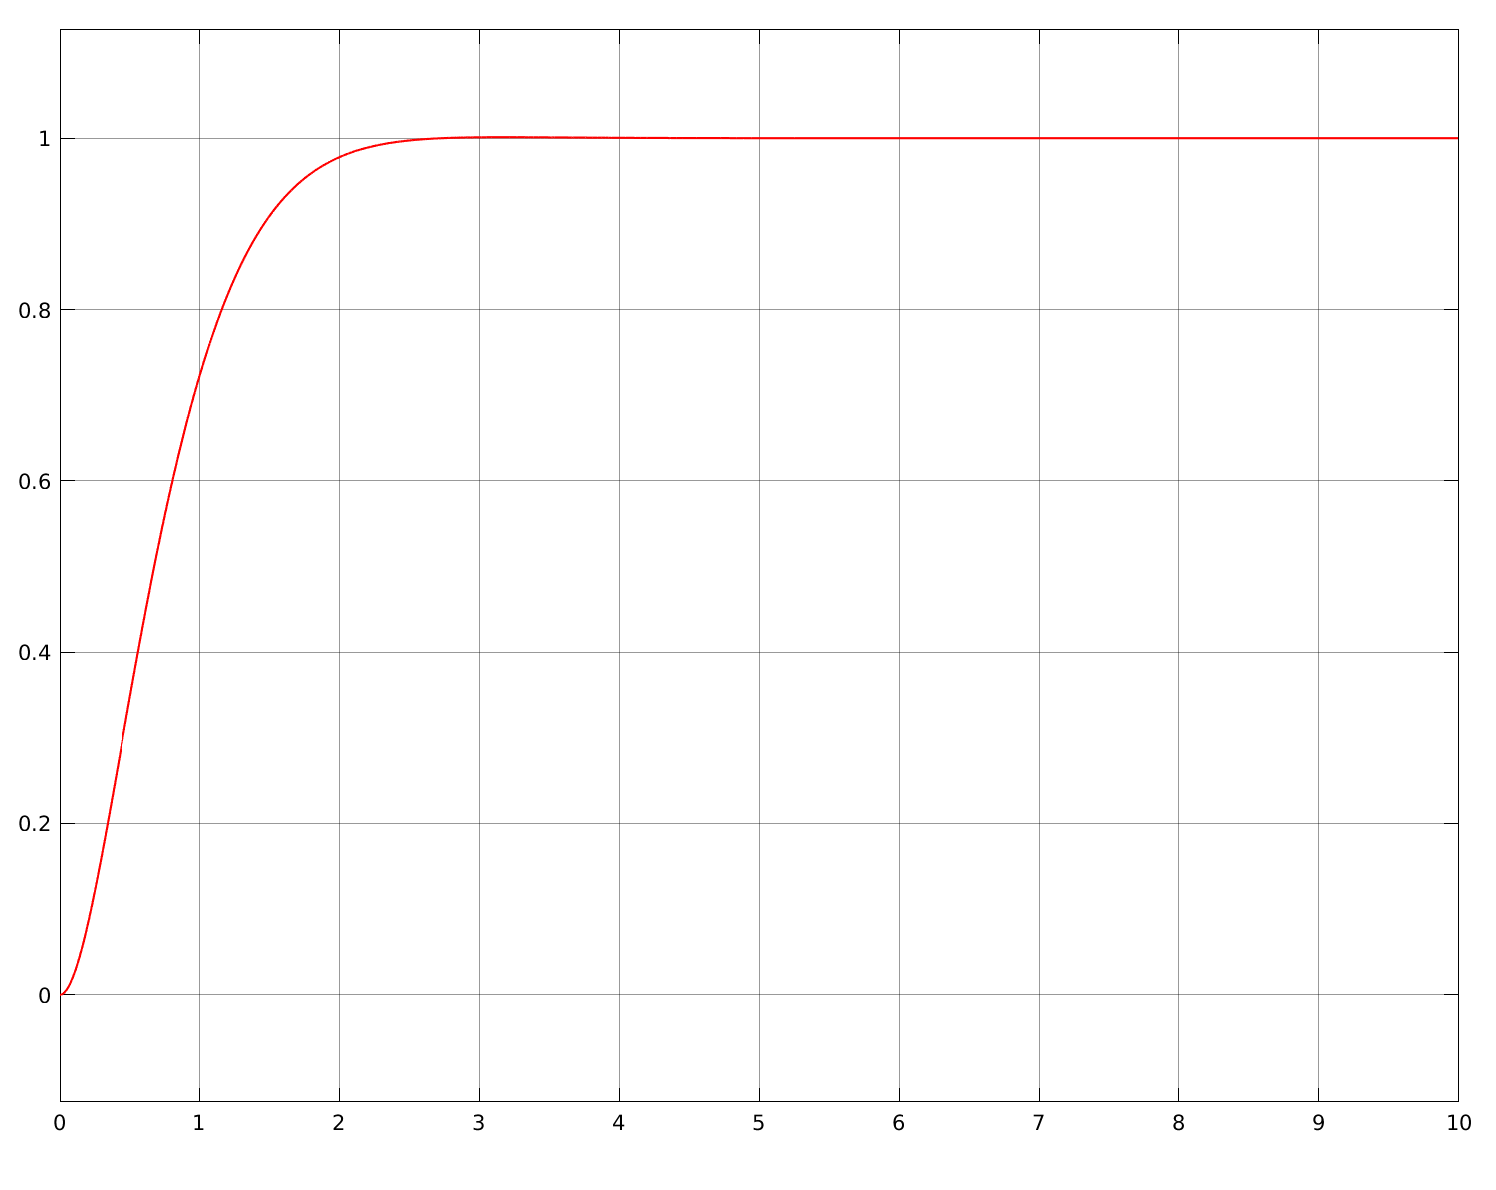
\includegraphics[scale=0.4]{q3_tuned_whole}
        \vspace*{-2mm}
        \caption{Tuned system reponse for Question 3}
    \end{figure}

    \begin{figure}[h]
        \centering
        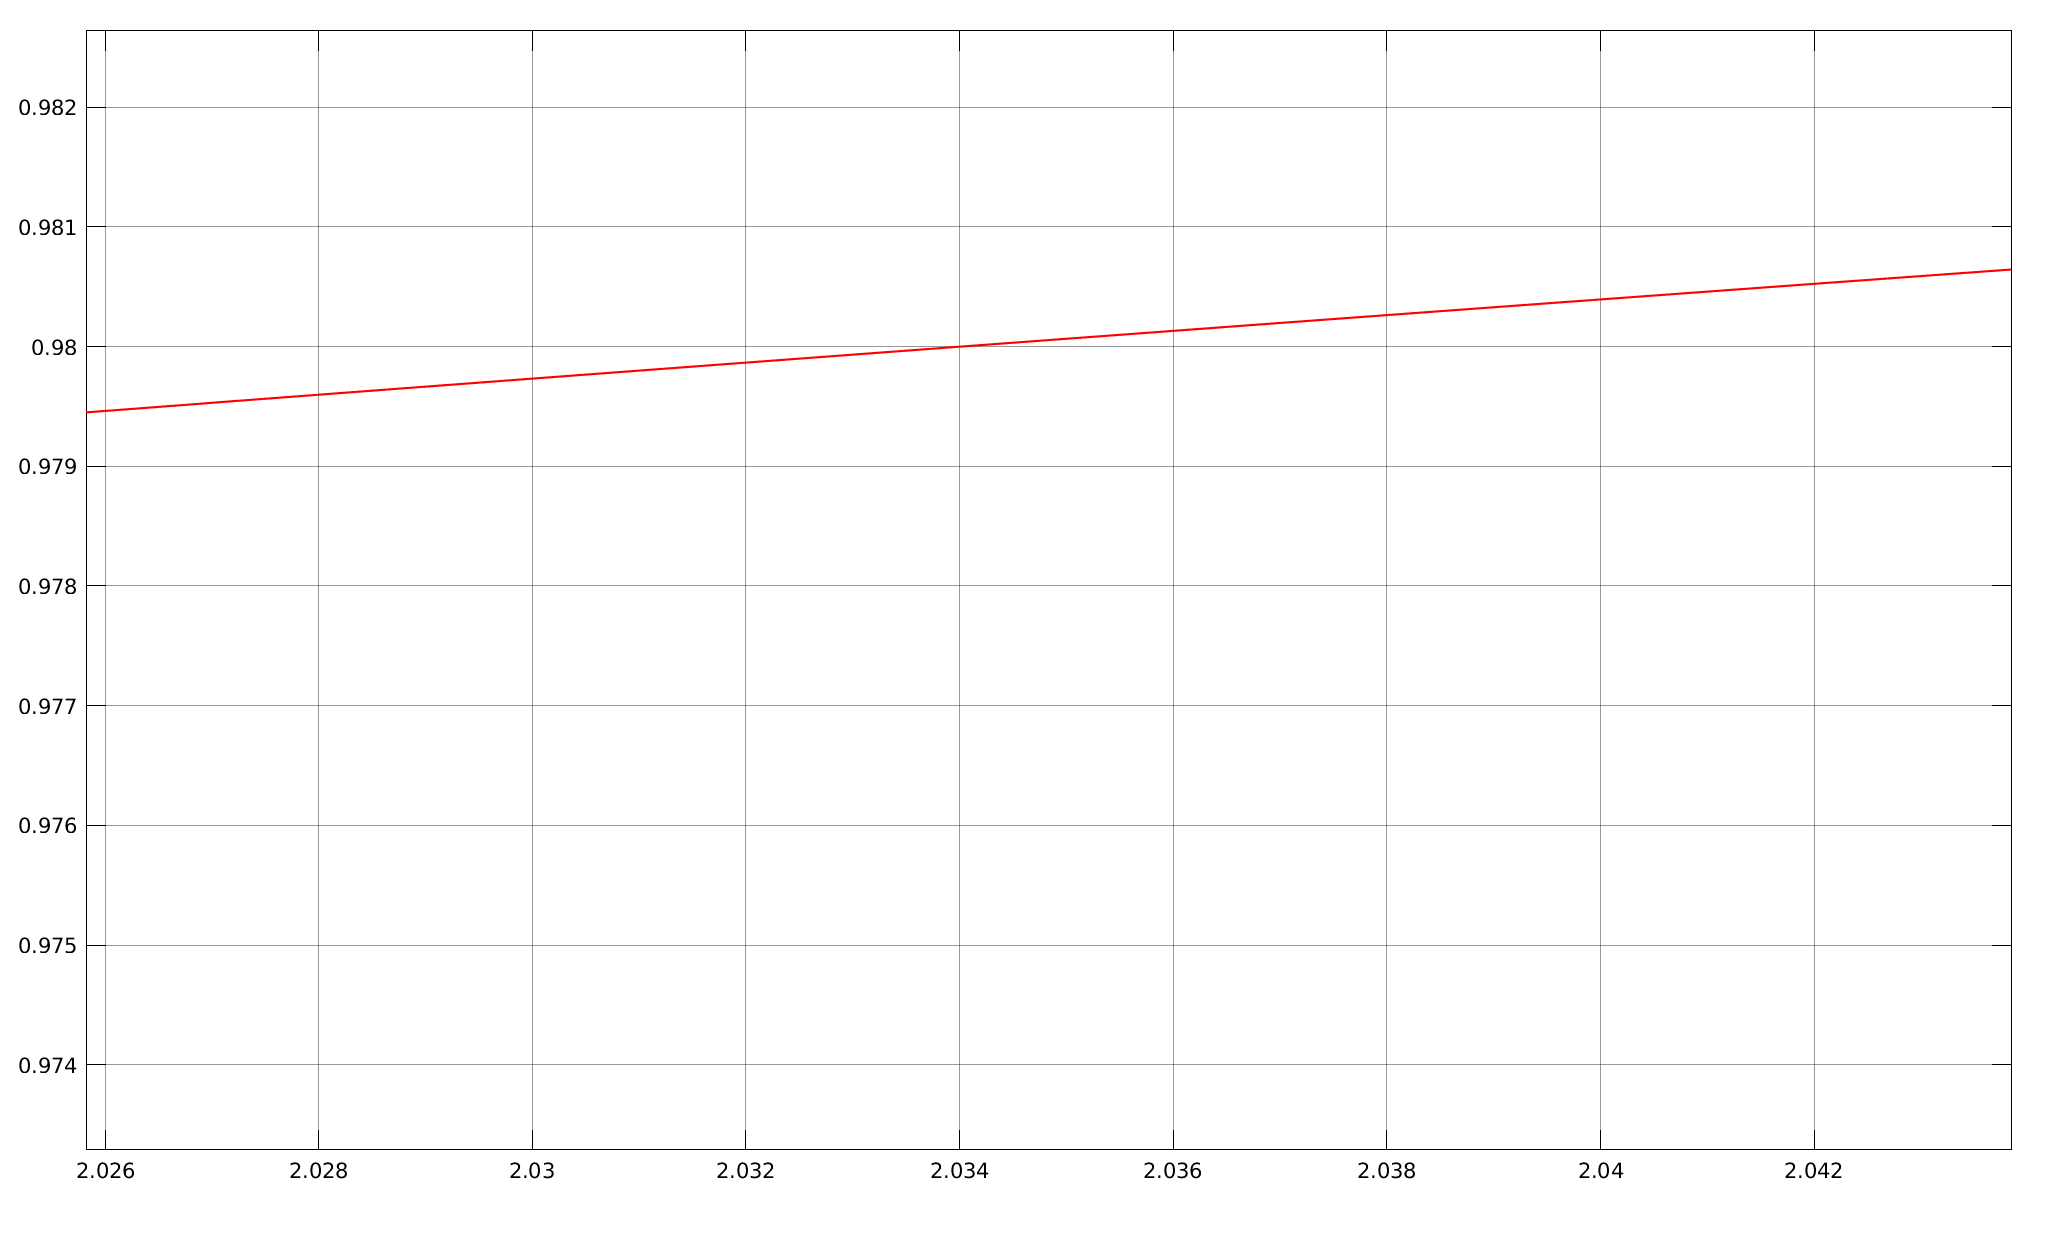
\includegraphics[scale=0.33]{q3_tuned_settling}
        \vspace*{-2mm}
        \caption{Zoomed-in plot to show settling time for Question 3}
    \end{figure}
    
\end{homeworkProblem}

\nobreak\extramarks{Question 4}{}\nobreak{}

\pagebreak

\begin{homeworkProblem}[Question 4]
    Now add a constant disturbance to the system, (Please check the lecture 
    slides for where to add this disturbance from to your simulink block diagram), by using “constant” 
    block from “Sources”. Assign the value $D$ to the block. Define this same parameter in the script 
    and set its value to $D = 0.5$. Provide the plot for theta with the same gain values to the previous 
    question. You will see some steady state error. Report the amount of steady state error. 

    \subsection{Solution}
    Our new block diagram, with disturbance $D$ added, is shown in Figure 6.

    \begin{figure}[h]
        \centering
        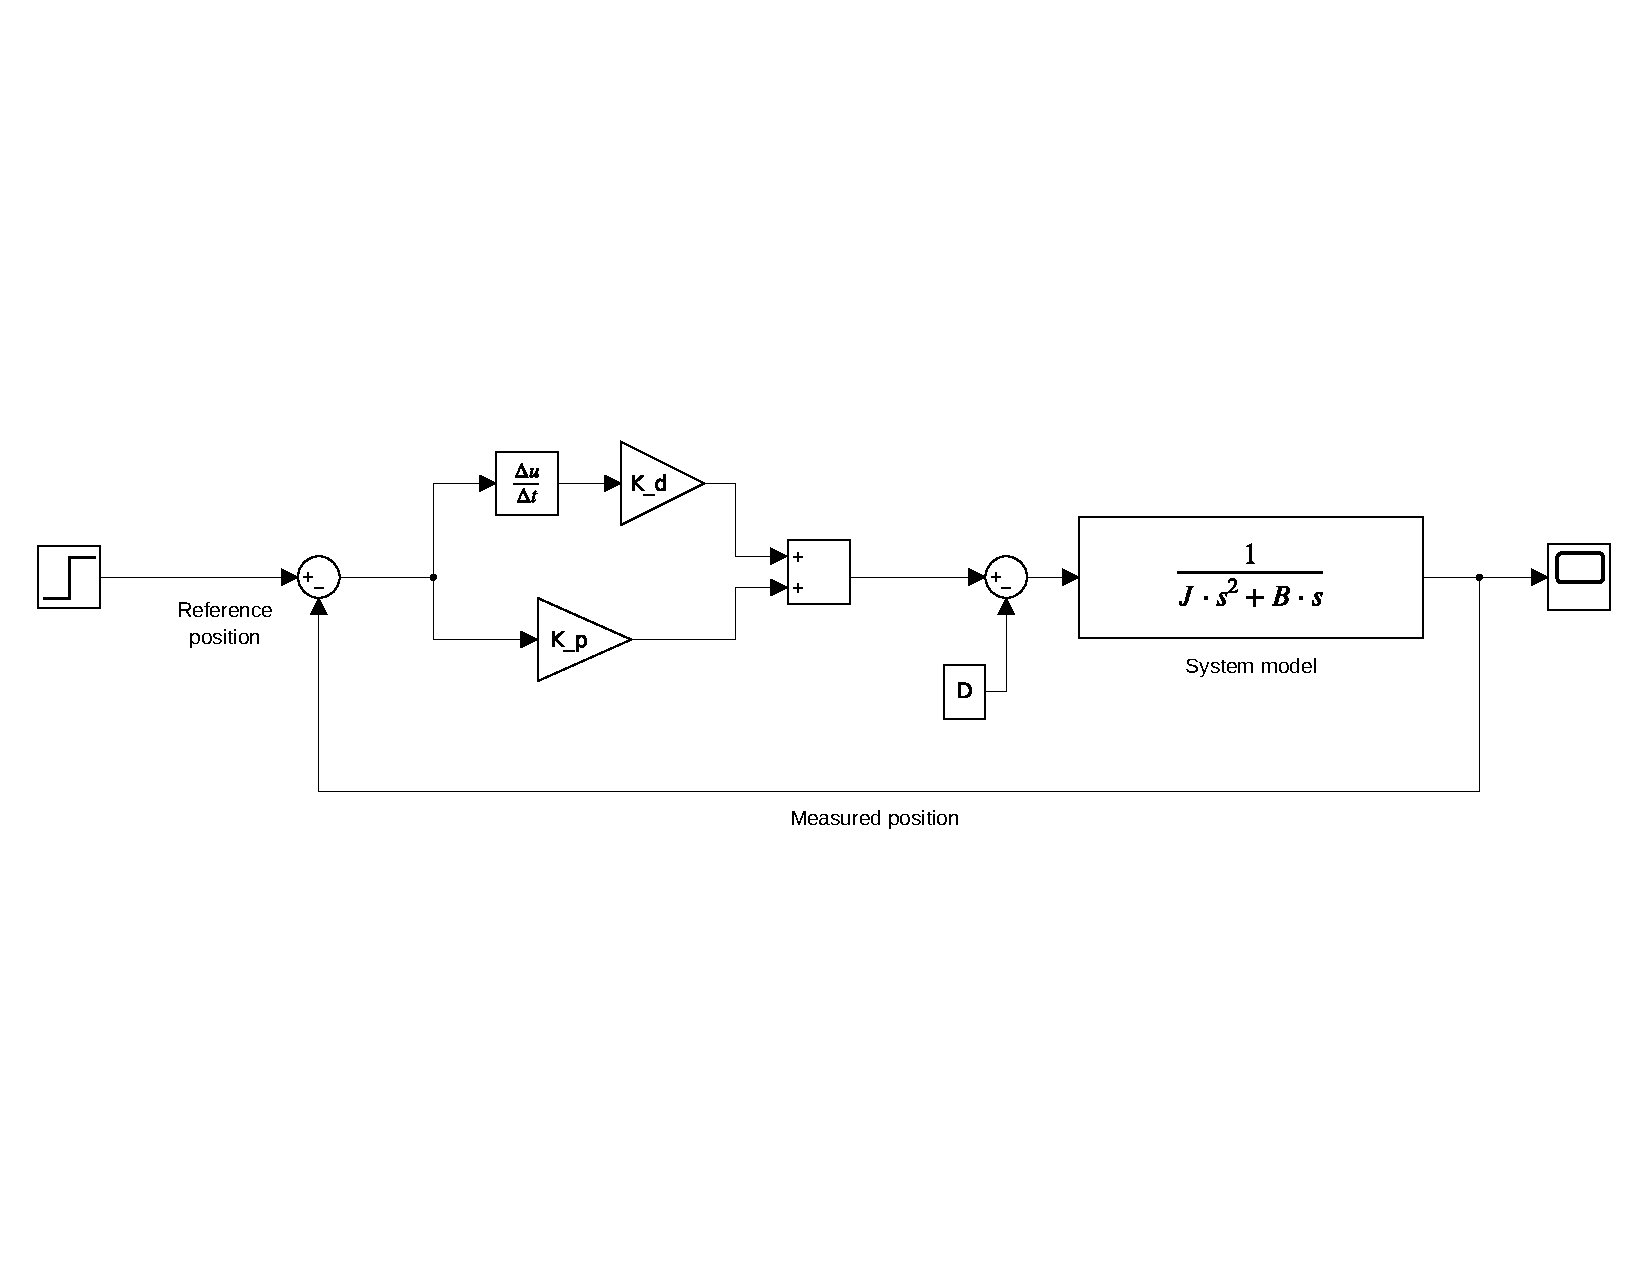
\includegraphics[scale=0.59]{hw6_system_disturbed}
        \vspace*{-7mm}
        \caption{Block diagram with disturbance}
    \end{figure}

    At this point, our MATLAB script looks as follows.

    \lstinputlisting{hw6_q4.m}

    \vspace{0.15in}

    Now we run our simulation again, and obtain the plot shown on the next page (Figure 7).

    \vspace{3in}

    \begin{figure}[h]
        \centering
        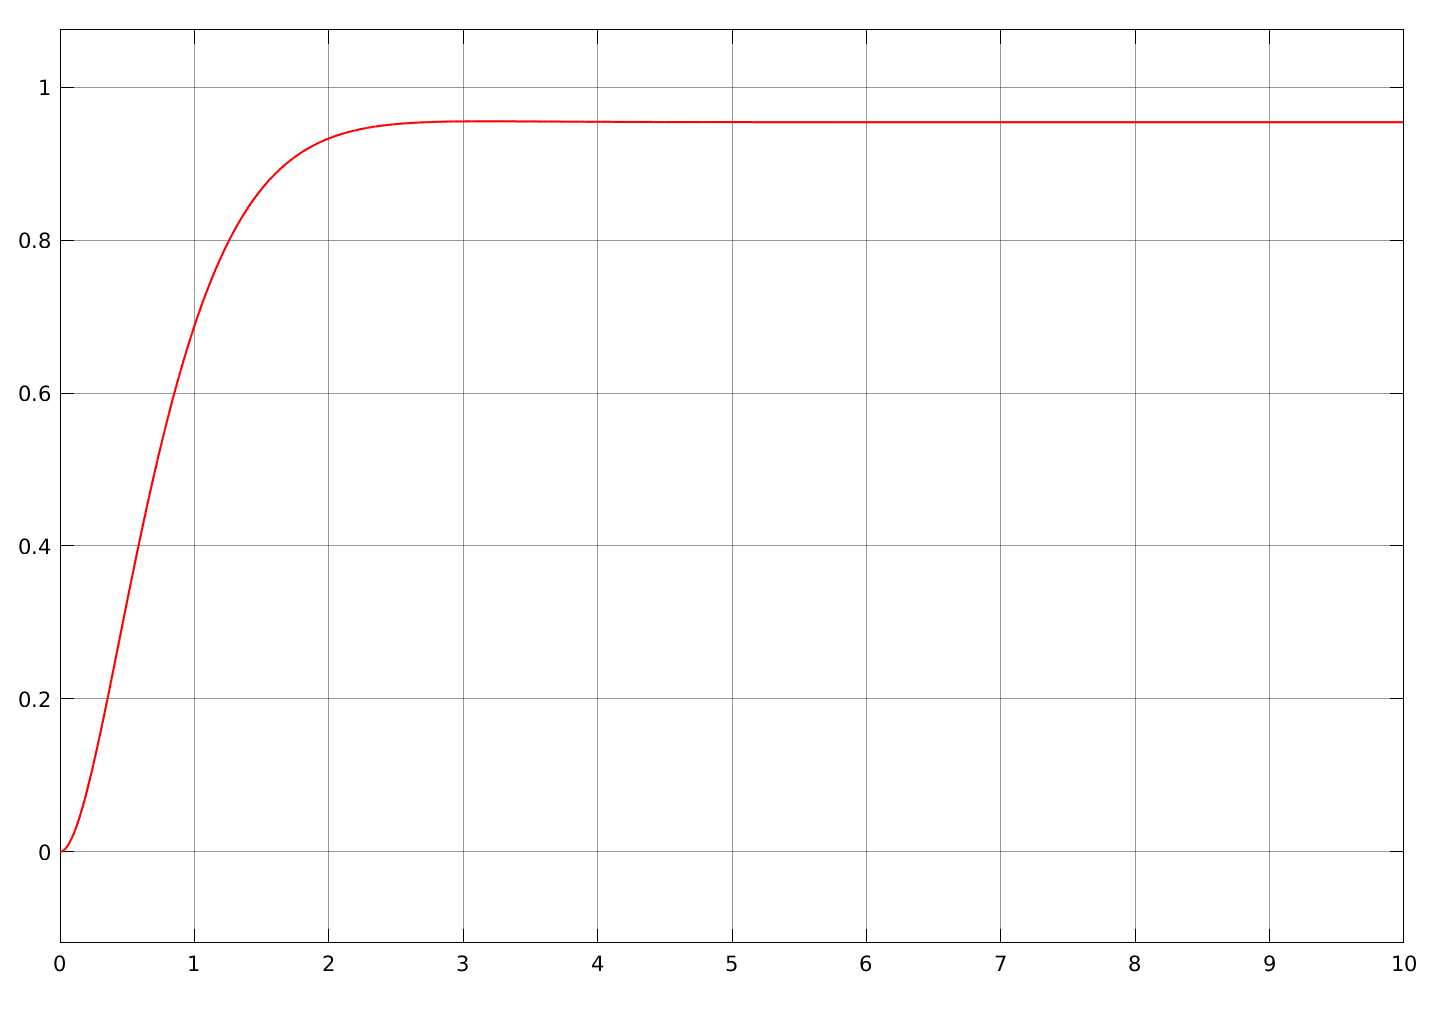
\includegraphics[scale=0.4]{q4_disturbance_plot}
        \vspace*{-2mm}
        \caption{Disturbed system reponse for Question 4}
    \end{figure}

    Clearly, there is a steady state error because the response stabilizes before it reaches the target value of 1. Therefore it is a negative error.\\
    \vspace{0mm}\\
    To see the magnitude of the error, let us zoom into the plot as shown in Figure 8.

    \begin{figure}[h]
        \centering
        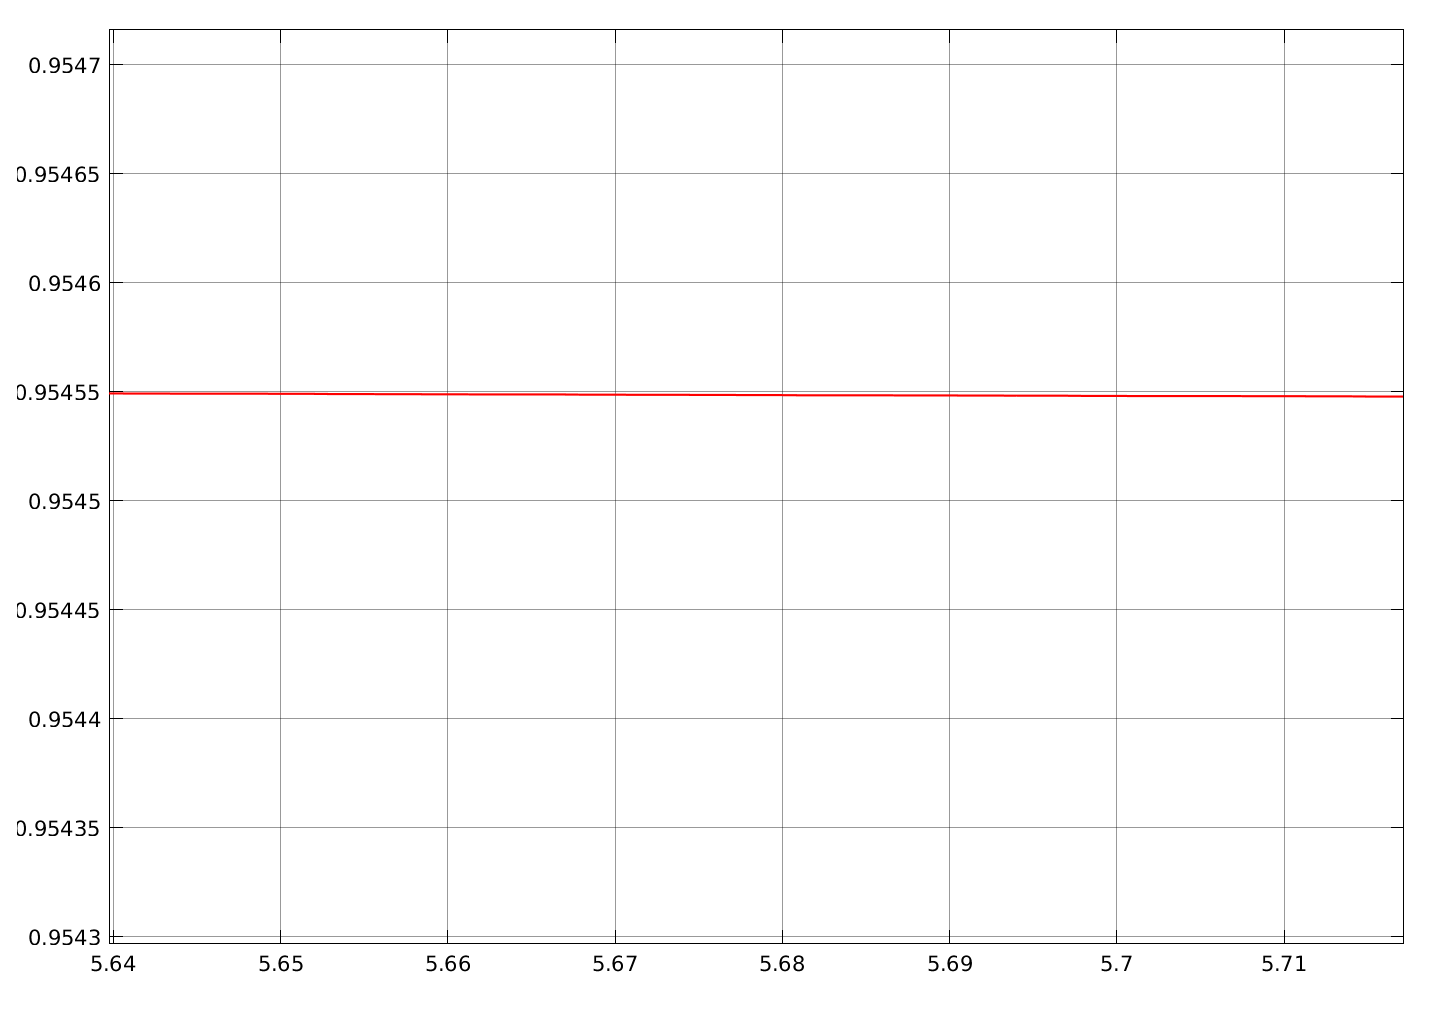
\includegraphics[scale=0.4]{q4_steady_state_err}
        \vspace*{-2mm}
        \caption{Disturbed system reponse for Question 4}
    \end{figure}

    This shows that the system settles around $0.95455$.\\

    Therefore, the steady state error is \(0.95455 - 1 = \boxed{-0.04545}\), or a \(\boxed{-4.545\%}\) error.
\end{homeworkProblem}

\nobreak\extramarks{Question 4}{}\nobreak{}

\pagebreak

\begin{homeworkProblem}[Question 5]
    Keeping the disturbance the same, add the integral term to your controller 
    (using  the  integral  Simulink  blocks)  and  tune  the  P,  I  and  D  gains  to  obtain  the  desired 
    performance and remove the steady state error even under the disturbance effect. Report the 
    current $K_p$, $K_d$ and $K_i$ values together with your new plot.  

    \subsection{Solution}

    First, we edit our MATLAB script so that it looks as follows.

    \lstinputlisting{hw6_q5.m}

    \vspace{0.15in}

    Now we edit our Simulink block diagram so that it looks as follows (Figure 9).

    \begin{figure}[h]
        \centering
        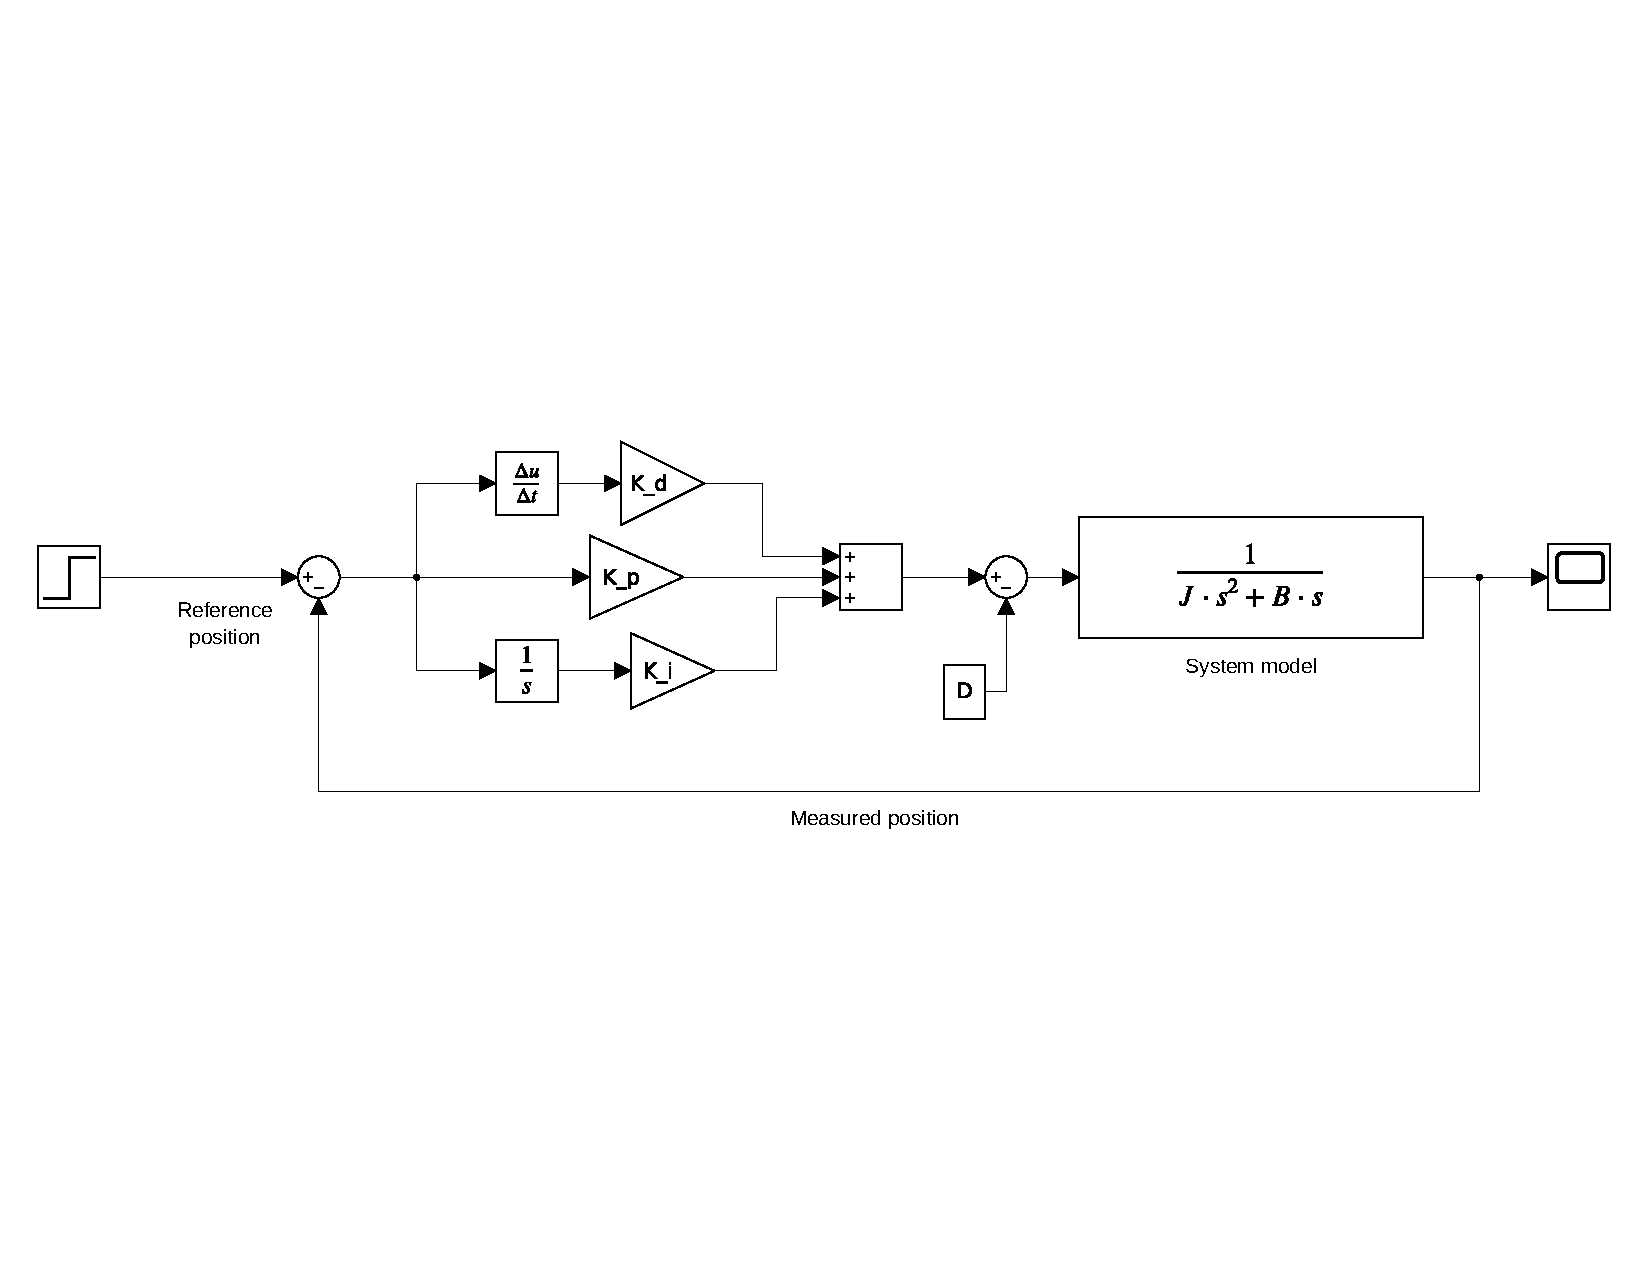
\includegraphics[scale=0.59]{hw6_system_pid}
        \vspace*{-7mm}
        \caption{Block diagram with PID controller}
    \end{figure}

\end{homeworkProblem}

\end{document}